\documentclass{beamer}
\usepackage[utf8]{inputenc}

\usetheme{Boadilla}
\usecolortheme{lily}
\usepackage{amsmath,amssymb,amsfonts,amsthm}
\usepackage{mathtools}
\usepackage{txfonts}
\usepackage{tkz-euclide}
\usepackage{listings}
\usepackage{adjustbox}
\usepackage{array}
\usepackage{tabularx}
\usepackage{lmodern}
\usepackage{gvv}
\usepackage{circuitikz}
\usepackage{tikz}
\usepackage{graphicx}

\setbeamertemplate{footline}
{
  \leavevmode%
  \hbox{%
  \begin{beamercolorbox}[wd=\paperwidth,ht=2.25ex,dp=1ex,right]{author in head/foot}%
    \insertframenumber{} / \inserttotalframenumber\hspace*{2ex} 
  \end{beamercolorbox}}%
  \vskip0pt%
}

\usepackage{tcolorbox}
\tcbuselibrary{minted,breakable,xparse,skins}




\providecommand{\nCr}[2]{\,^{#1}C_{#2}} % nCr
\providecommand{\nPr}[2]{\,^{#1}P_{#2}} % nPr
\providecommand{\mbf}{\mathbf}
\providecommand{\pr}[1]{\ensuremath{\Pr\left(#1\right)}}
\providecommand{\qfunc}[1]{\ensuremath{Q\left(#1\right)}}
\providecommand{\sbrak}[1]{\ensuremath{{}\left[#1\right]}}
\providecommand{\lsbrak}[1]{\ensuremath{{}\left[#1\right.}}
\providecommand{\rsbrak}[1]{\ensuremath{{}\left.#1\right]}}
\providecommand{\brak}[1]{\ensuremath{\left(#1\right)}}
\providecommand{\lbrak}[1]{\ensuremath{\left(#1\right.}}
\providecommand{\rbrak}[1]{\ensuremath{\left.#1\right)}}
\providecommand{\cbrak}[1]{\ensuremath{\left\{#1\right\}}}
\providecommand{\lcbrak}[1]{\ensuremath{\left\{#1\right.}}
\providecommand{\rcbrak}[1]{\ensuremath{\left.#1\right\}}}
\theoremstyle{remark}
\newcommand{\sgn}{\mathop{\mathrm{sgn}}}
\providecommand{\abs}[1]{\left\vert#1\right\vert}
\providecommand{\res}[1]{\Res\displaylimits_{#1}} 
\providecommand{\norm}[1]{\lVert#1\rVert}
\providecommand{\mtx}[1]{\mathbf{#1}}
\providecommand{\mean}[1]{E\left[ #1 \right]}
\providecommand{\fourier}{\overset{\mathcal{F}}{ \rightleftharpoons}}
%\providecommand{\hilbert}{\overset{\mathcal{H}}{ \rightleftharpoons}}
\providecommand{\system}{\overset{\mathcal{H}}{ \longleftrightarrow}}
	%\newcommand{\solution}[2]{\textbf{Solution:}{#1}}
%\newcommand{\solution}{\noindent \textbf{Solution: }}
\providecommand{\dec}[2]{\ensuremath{\overset{#1}{\underset{#2}{\gtrless}}}}
\newcommand{\myvec}[1]{\ensuremath{\begin{pmatrix}#1\end{pmatrix}}}
\let\vec\mathbf

\lstset{
%language=C,
frame=single, 
breaklines=true,
columns=fullflexible
}

\numberwithin{equation}{section}

\lstset{
  language=Python,
  basicstyle=\ttfamily\small,
  keywordstyle=\color{blue},
  stringstyle=\color{orange},
  numbers=left,
  numberstyle=\tiny\color{gray},
  breaklines=true,
  showstringspaces=false
}

\title{Problem 10.7.72}
\author{ee25btech11023-Venkata Sai}

\date{\today} 
\begin{document}

\begin{frame}
\titlepage
\end{frame}

\section*{Outline}
\begin{frame}
\tableofcontents
\end{frame}

\section{Problem}

\begin{frame}
\frametitle{Problem}
The chords of contact of the pair of tangents drawn from each point on the line
$2x + y = 4$ to $x^2 + y^2 = 1 $ pass through the point $\dots$
\end{frame}
%\subsection{Literature}
\section{Solution}

 
\subsection{Equation}
\begin{frame}
\frametitle{Equation}
The general equation of conic
\begin{align}
    \vec{x}^\top\vec{V}\vec{x} + 2\vec{u}^\top\vec{x} + f = 0
\end{align}
The chord of contact of tangents from an external point $\vec{q}$ is given by
\begin{align}
 \brak{\vec{V}\vec{q}+\vec{u}}^\top\vec{x}+\vec{u}^\top\vec{q}+f=0
\end{align}
Given circle in matrix form
\begin{align}
x^2 + y^2 &= 1  \\
x^2 + y^2 - &1=0 \\
\vec{x}^\top\myvec{1 &0 \\0 &1}\vec{x}&-1=0
\end{align}
where
\begin{align}
\vec{V}=\myvec{1&0\\0&1}=\vec{I},\vec{u}=\vec{0},f=-1
\end{align}
\end{frame}
\subsection{Simplify}
\begin{frame}
\frametitle{Simplify}
Given line 
\begin{align}
2x + y = 4 \\ 
\myvec{2&1}\vec{x}=4
\end{align}
As $\vec{q}$ satisfies \brak{8}
\begin{align}
   \myvec{2&1}\vec{q}=4 
\end{align}
From \brak{2} and \brak{6}
\begin{align}
  \brak{\vec{I}\vec{q}+\vec{0}}^\top\vec{x}&+\vec{0}^\top\vec{q}-1=0 \\
  \brak{\vec{I}\vec{q}}^\top\vec{x}&-1=0\\
  \vec{q}^\top\vec{x}&-1=0\\
  \vec{q}^\top\vec{x}=1&\implies
  \vec{x}^\top\vec{q}=1 
  \end{align}
From \brak{9} and \brak{13}
 \end{frame}
 \subsection{Conclusion}
\begin{frame}
\frametitle{Conclusion}
\begin{align}
    \vec{x}^\top&=k\myvec{2&1}\\
    \brak{k\myvec{2&1}}^\top\vec{q}=1&\implies
    k\myvec{2&1}^\top\vec{q}=1\\
    k\brak{4}=1 &\implies k=\frac{1}{4} \\
\vec{x}^\top=\frac{1}{4}\myvec{2&1} &\implies \vec{x}^\top=\myvec{\frac{1}{2}&\frac{1}{4}}\\
    \vec{x}&=\myvec{\frac{1}{2}\\\frac{1}{4}}
\end{align}
Hence the chords of contact pass through the point  $\myvec{\frac{1}{2}\\\frac{1}{4}}$
 \end{frame}
\subsection{Plot}
\begin{frame}[fragile]
\frametitle{Plot}

\begin{figure}[h!]
   \centering
   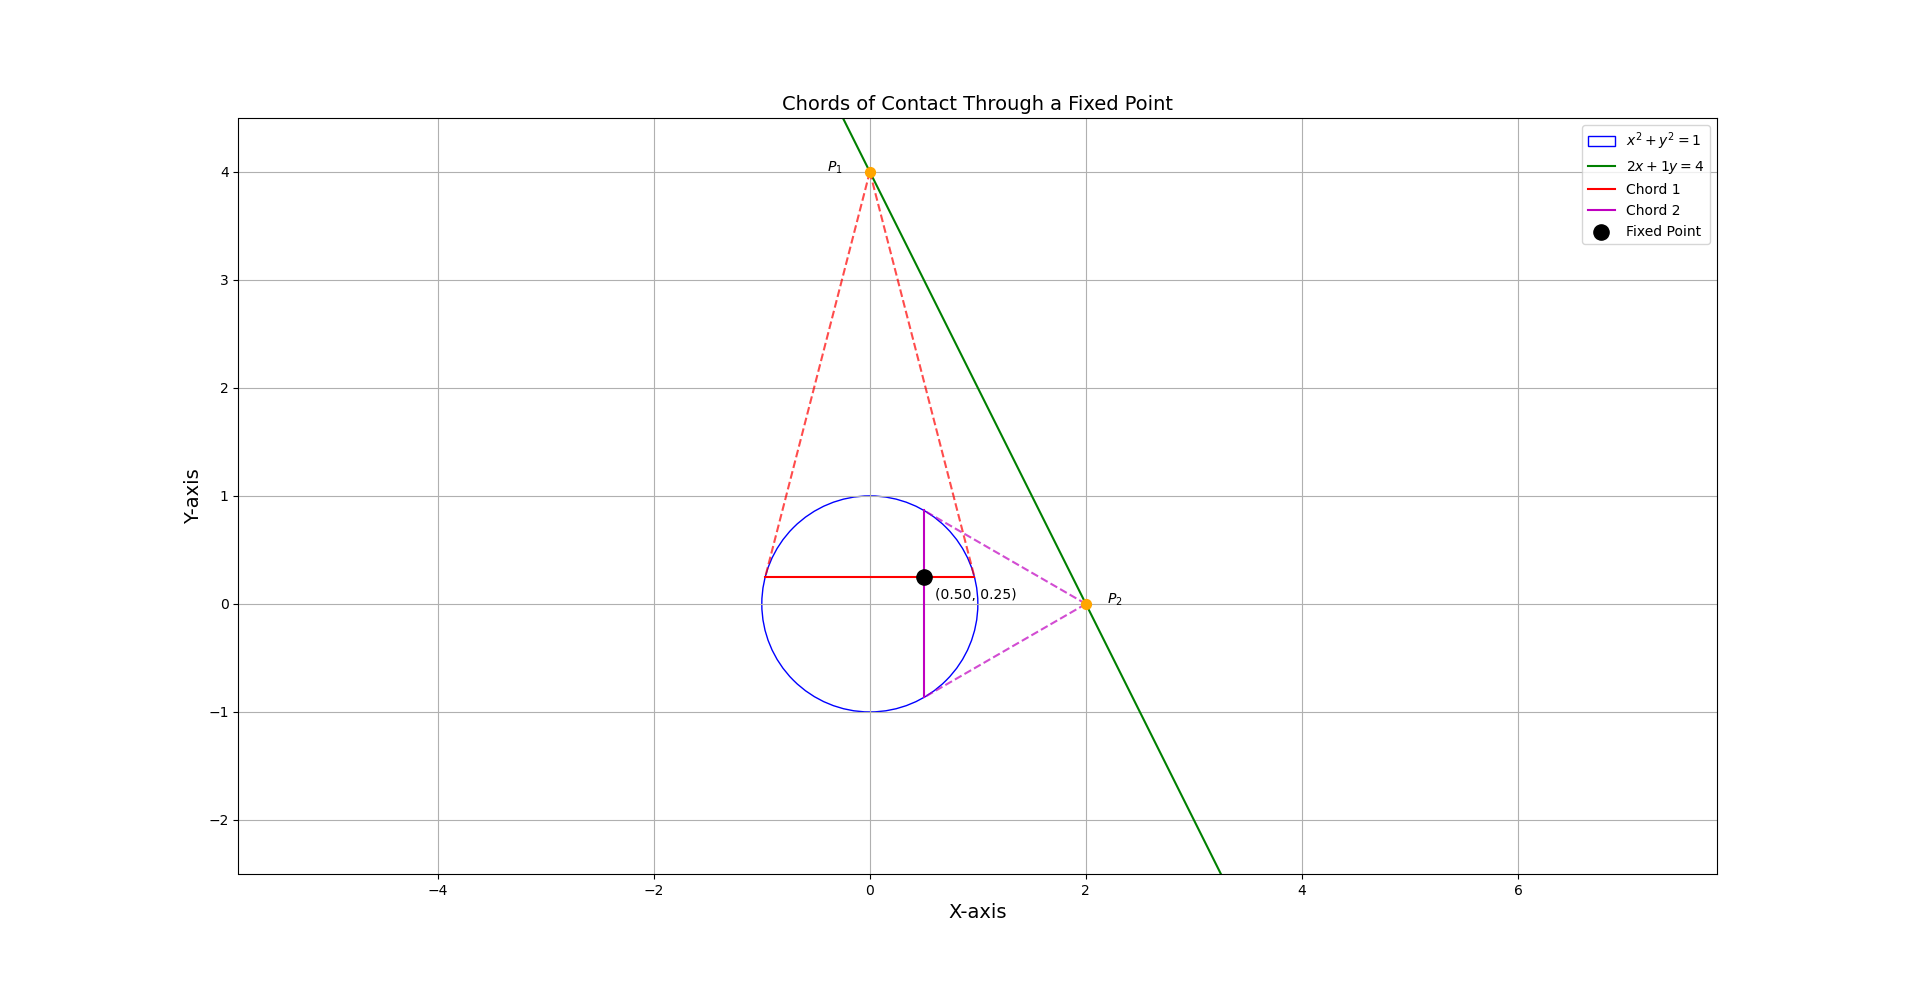
\includegraphics[width=0.9\columnwidth]{figs/fig1.png}
	\caption{}
   \label{}
\end{figure}
\end{frame}

\section{C Code}
\begin{frame}[fragile]
\frametitle{C Code}
\begin{lstlisting}[language=C]
void get_problem_data(double* out_data) {
    out_data[0] = 2.0;
    out_data[1] = 1.0;
    out_data[2] = -4.0;
    out_data[3] = 1.0;
}


    \end{lstlisting}
\end{frame}

\section{Python Code}
\begin{frame}[fragile]
\frametitle{Python Code for Solving}
\begin{lstlisting}[language=Python]
import ctypes
import numpy as np
import sympy as sp

def get_plot_data():

    lib = ctypes.CDLL('./code.so')
    out_data = (ctypes.c_double * 4)()
    lib.get_problem_data(out_data)
    a, b, c, r = list(out_data)

    x, y, x0, y0 = sp.symbols('x y x0 y0')
    y0_expr = sp.solve(a*x0 + b*y0 + c, y0)[0]
    chord_on_line = (x*x0 + y*y0 - r**2).subs(y0, y0_expr)
    poly = sp.Poly(chord_on_line, x0)

    eq1 = poly.coeff_monomial(x0)
    eq2 = poly.coeff_monomial(1)
\end{lstlisting}
\end{frame}
 \begin{frame}[fragile]
\frametitle{Python Code for Solving}
\begin{lstlisting} 
sol = sp.solve([eq1, eq2], [x, y])
    p_fixed = np.array([float(sol[x]), float(sol[y])])

    p1 = np.array([0.0, 4.0])
    p2 = np.array([2.0, 0.0])

    t1 = np.array([np.sqrt(15)/4, 1/4])
    t2 = np.array([-np.sqrt(15)/4, 1/4])
    t3 = np.array([1/2, np.sqrt(3)/2])
    t4 = np.array([1/2, -np.sqrt(3)/2])

    return {
        "p_fixed": p_fixed,
        "p1": p1, "t1": t1, "t2": t2,
        "p2": p2, "t3": t3, "t4": t4,
        "line_coeffs": (a, b, c)
    }
\end{lstlisting}
\end{frame}
 
\begin{frame}[fragile]
\frametitle{Python Code for Plotting}
\begin{lstlisting}[language=Python]
# Code by /sdcard/github/matgeo/codes/CoordGeoVV Sharma
# September 12, 2023
# Revised July 21, 2024
# Released under GNU GPL
# Section Formula
import sys
sys.path.insert(0, '/workspaces/urban-potato/matgeo/codes/CoordGeo/') 
import matplotlib.pyplot as plt
import numpy as np
from call import get_plot_data

data = get_plot_data()
P = data["p_fixed"]
P1, T1, T2 = data["p1"], data["t1"], data["t2"]
P2, T3, T4 = data["p2"], data["t3"], data["t4"]
a, b, c = data["line_coeffs"]

fig, ax = plt.subplots(figsize=(9, 9))


\end{lstlisting}
\end{frame}
\begin{frame}[fragile]
\frametitle{Python Code for Plotting}
\begin{lstlisting}[language=Python]

circle = plt.Circle((0, 0), 1, color='blue', fill=False, label='$x^2+y^2=1$')

ax.add_patch(circle)
x_vals = np.array([-1, 4])
y_vals = (-a * x_vals - c) / b
ax.plot(x_vals, y_vals, 'g-', label=f'${int(a)}x+{int(b)}y={int(-c)}$')
ax.plot([P1[0], T1[0]], [P1[1], T1[1]], 'r--', alpha=0.7)
ax.plot([P1[0], T2[0]], [P1[1], T2[1]], 'r--', alpha=0.7)
ax.plot([T1[0], T2[0]], [T1[1], T2[1]], 'r-', label='Chord 1')

ax.plot([P2[0], T3[0]], [P2[1], T3[1]], 'm--', alpha=0.7)
ax.plot([P2[0], T4[0]], [P2[1], T4[1]], 'm--', alpha=0.7)
ax.plot([T3[0], T4[0]], [T3[1], T4[1]], 'm-', label='Chord 2')

ax.scatter([P1[0], P2[0]], [P1[1], P2[1]], color='orange', s=50, zorder=5)

           
\end{lstlisting}
\end{frame}
 \begin{frame}[fragile]
\frametitle{Python Code for Plotting}
\begin{lstlisting}[language=Python]
ax.text(P1[0] - 0.4, P1[1], '$P_1$')
ax.text(P2[0] + 0.2, P2[1], '$P_2$')

ax.scatter(P[0], P[1], color='black', s=120, zorder=5, label='Fixed Point')
ax.text(P[0] + 0.1, P[1] - 0.2, f'({P[0]:.2f}, {P[1]:.2f})')

ax.set_title('Chords of Contact Through a Fixed Point')
ax.set_xlabel('X-axis'); ax.set_ylabel('Y-axis')
ax.text(P1[0] - 0.4, P1[1], '$P_1$')
ax.text(P2[0] + 0.2, P2[1], '$P_2$')

ax.scatter(P[0], P[1], color='black', s=120, zorder=5, label='Fixed Point')
ax.text(P[0] + 0.1, P[1] - 0.2, f'({P[0]:.2f}, {P[1]:.2f})')

ax.set_title('Chords of Contact Through a Fixed Point')
ax.set_xlabel('X-axis'); ax.set_ylabel('Y-axis')
\end{lstlisting}
\end{frame}
\end{document}
